\section{Gradual Permission Regions}

\begin{figure}[t]
\centering
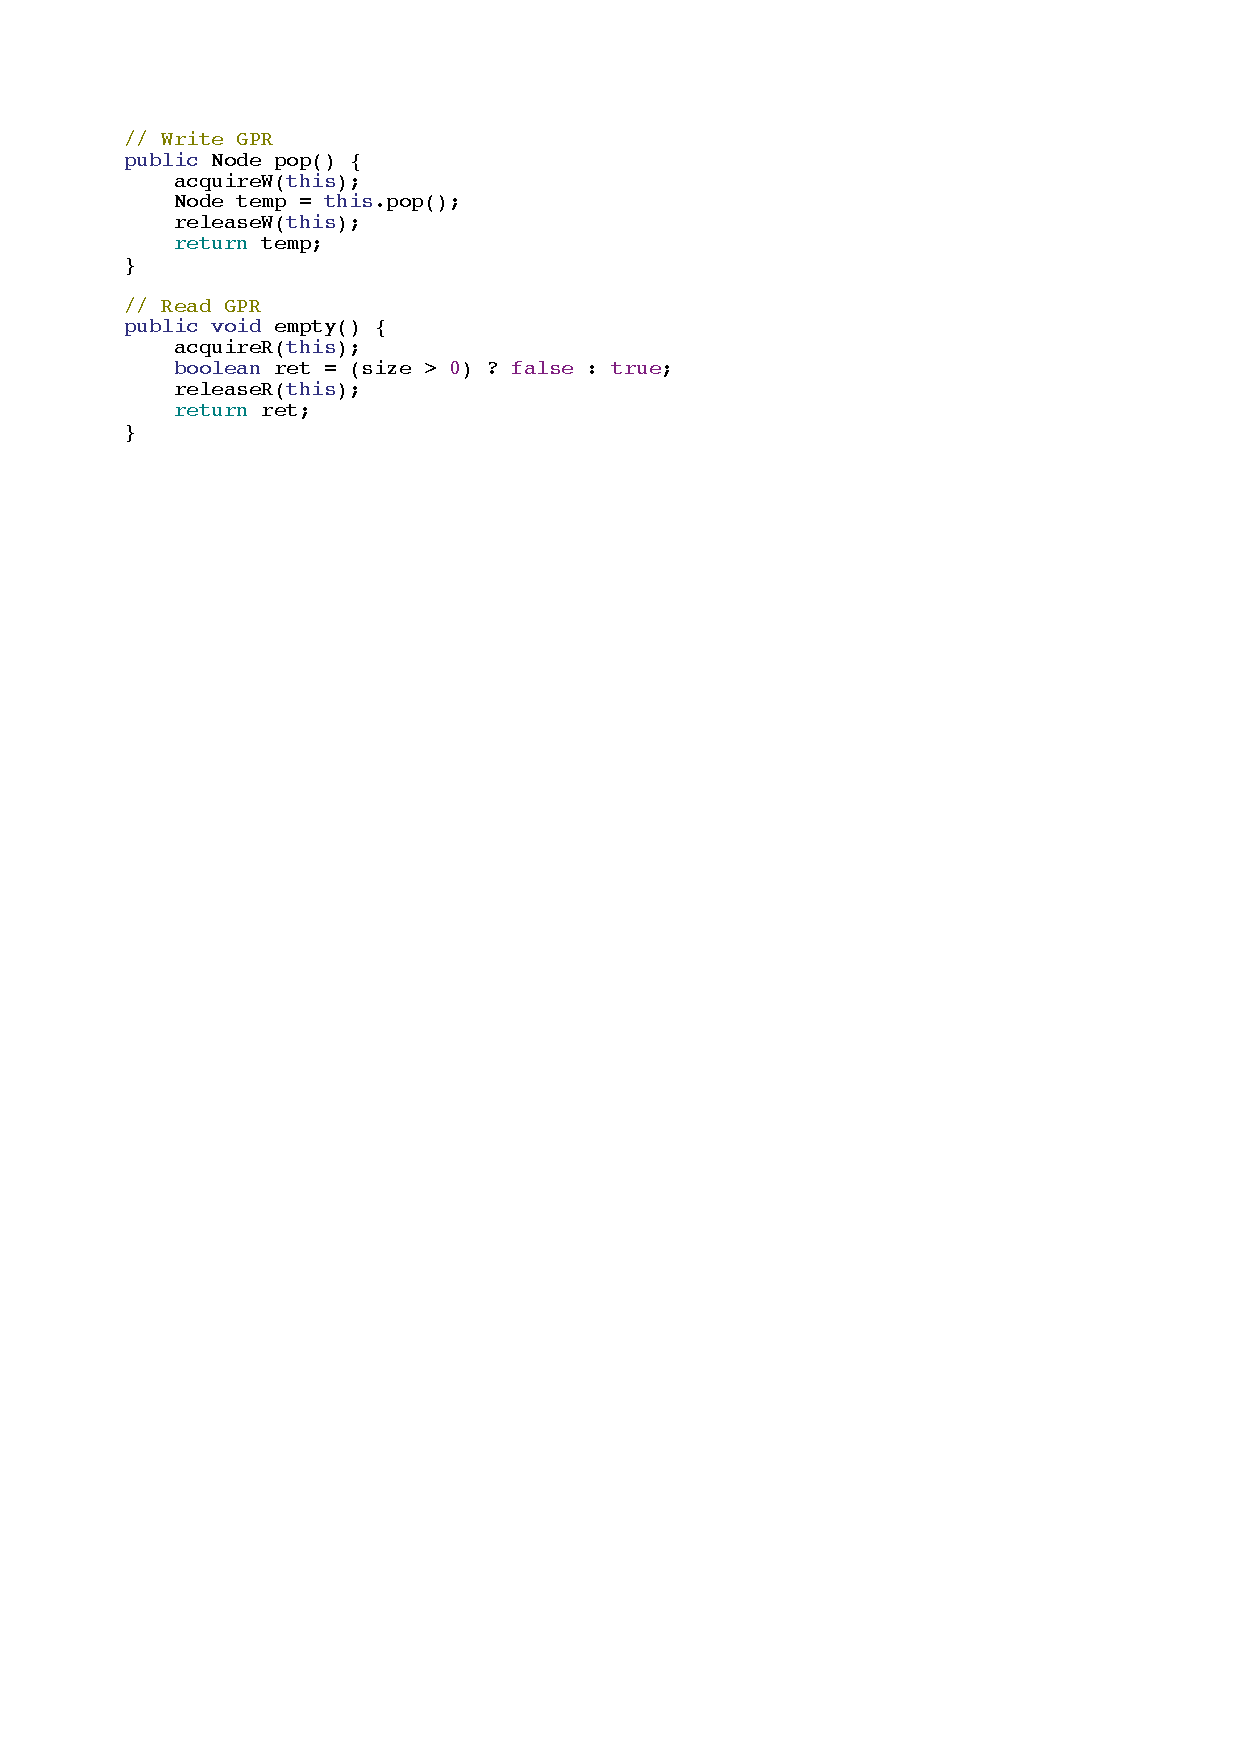
\includegraphics[width=3.25in]{../figs/gpr.pdf}
\caption{Stack methods integrated with GPRs}
\label{fig:gpr-read-write}
\end{figure}

GPRs function much like traditional race detection
tools\cite{Westbrook:2011:PRR:2341616.2341627,Westbrook:2012:PPR:2367163.2367201}.
However, the granularity of the dynamic checks is increased to sections of code
instead of individual memory accesses. GPRs annotate variables over sections of
code with either read or write permissions. Concurrent execution of tasks within
two or more conflicting GPRs is detected at runtime as a violation of GPR rules
and an exception is thrown. Conflicting GPRs are defined as regions that access
the same variable with at least one of the regions being a "write" region.  In
general, GPRs can be used to annotate over multiple variables including
parameters of a method with a single annotation. VR-lib does not yet support
this feature. To protect multiple variables, multiple annotations must be used.

In VR-lib, a GPR is delimited by {\tt acquireR/acquireW (Object X)} at the beginning
and {\tt releaseR/releaseW (Object X)} atthe end of a region,
with R/W representing read and write respectively. A correctly annotated region
uses the same object reference in the corresponding acquire/release statements.
See \figref{fig:gpr-read-write} for an example of using GPRs to annotate methods
in a class. Note that the acquire/release calls are assertions of permissions rather than actions. A call to acquireR/acquireW asserts that it is
safe to read/write the specified object in the region of code until the matching
releaseR/releaseW call is encountered (unlike monitor-enter/monitor-exit
operations on locks which perform operations in support of mutual exclusion).
Thus, the verification problem becomes one of ensuring that no
acquireR/acquireW call results in a permission exception. The standard data race
detection problem can be modeled by wrapping each read/write operation in a
separate permission region. Larger permission regions enable checking of
invariants related to higher-level race conditions (while also guaranteeing the
absence of low-level races), and---as a bonus---are amenable to more efficient
verification than standard data race detection.

Our contribution to the work using GPRs is the implementation of GPRs within
VR-lib, which allows for the utilization of JPF to perform dynamic checks for
all legal schedules (for a given input). Thus, an HJ program, in which each
shared variable is guarded by a GPRs annotation, can be verified by JPF to be
free of race conditions. As a reminder, there are two important semantic
guarantees for a large subset of HJ programs (those that use async, finish,
future, or phaser constructs, but do not use isolated, actor, or data-driven
tasks). First, if any program in this subset is guaranteed to be data race
free, then it is also guaranteed to be determinate (functionally deterministic
and structurally deterministic) \cite{determinacy}. Second, all programs in
this subset are guaranteed to be deadlock-free. 

 
